\documentclass[12pt, a4paper]{article}

%%%%%%%%%%%%%%%引入Package%%%%%%%%%%%%%%%
\usepackage[margin=3cm]{geometry} % 上下左右距離邊緣2cm
\usepackage{amsmath,amsthm,amssymb} % 引入 AMS 數學環境   
%\usepackage{algpseudocode}

\usepackage{listings}
\usepackage{algorithm}
\usepackage{algorithmic}
\usepackage{yhmath}      % math symbol
\usepackage{graphicx}    % 圖形插入用
%\usepackage{forest}
%\graphicspath{{images/}}  % 搜尋圖片目錄
\usepackage{wrapfig}     % 文繞圖
\usepackage{subcaption}
%\usepackage{floatflt}    % 浮動 figure
%\usepackage{float}       % 浮動環境
%\usepackage{subfig}      % subfigures
%\usepackage{caption3}    % caption 增強
%\usepackage{setspace}    % 控制空行
\usepackage{fontspec}    % 加這個就可以設定字體
\usepackage{type1cm}	 % 設定fontsize用
\usepackage{titlesec}   % 設定section等的字體
\usepackage{titling}    % 加強 title 功能
\usepackage{fancyhdr}   % 頁首頁尾
\usepackage{tabularx}   % 加強版 table
\usepackage[square, comma, numbers, super, sort&compress]{natbib}% cite加強版
\usepackage[unicode=true, pdfborder={0 0 0}, bookmarksdepth=-1]{hyperref}% ref加強版
%\usepackage{soul}       % highlight
%\usepackage{ulem}       % 字加裝飾
\usepackage[usenames, dvipsnames]{color}  % 可以使用顏色
%\usepackage{framed}     % 可以加文字方框
\usepackage{enumerate}  % 加強版enumerate
\usepackage{enumitem}




%%%%%%%%%%%%%%中文 Environment%%%%%%%%%%%%%%%
\usepackage{xeCJK}  % xelatex 中文
%\usepackage{CJKulem}	% 中文字裝飾
\setCJKmainfont[AutoFakeBold=3,AutoFakeSlant=.4]{BiauKai}
\defaultCJKfontfeatures{AutoFakeBold=3,AutoFakeSlant=.4}
\newCJKfontfamily\Kai{BiauKai}
\newCJKfontfamily\Hei{微軟正黑體}
\newCJKfontfamily\NewMing{新細明體}
%設定中文為系統上的字型,而英文不去更動,使用原TeX字型

\XeTeXlinebreaklocale "zh"            
\XeTeXlinebreakskip = 0pt plus 1pt

\lstset{numbers=left, numberstyle=\tiny, stepnumber=1, numbersep=10pt}
\lstset{basicstyle=\ttfamily\footnotesize,breaklines=true, tabsize=4}

\usepackage{color}




%%%%%%%%%%%%%%%頁面設定%%%%%%%%%%%%%%%
\setlength{\headheight}{15pt}  %with titling
\setlength{\droptitle}{-1.5cm} %title 與上緣的間距
\parindent=24pt %設定縮排的距離
%\parskip=1ex  %設定行距
%\pagestyle{empty}  % empty: 無頁碼
\pagestyle{fancy}  % fancy: fancyhdr

%use with fancygdr
\lhead{}
%\chead{}
\rhead{}
\lfoot{}
%\cfoot{}
%\rfoot{\thepage}
%\renewcommand{\headrulewidth}{0.4pt}
%\renewcommand{\footrulewidth}{0.4pt}


%%%% above are environment settings %%%%


\begin{document}
\thispagestyle{fancy}  %使用fancyhdr
\fontsize{12pt}{24pt}\selectfont

%%%%%%%%%%%%%%%%%%%include file here%%%%%%%%%%%%%%%%%%%%%%%%%
%\let\clearpage\relax
\title{Fundamental Object Oriented Programming 2021 \\ Final Project \\ \textbf{Make It On Time}} %標題
\author{
    李宜璟\\B07401012\\
    \and
    陳冠廷\\B07902025\\
    \and
    陳倢堂\\B07902018\\
    \and
    鄭仲語\\B07508005\\
}
\date{Summer 2021}
\begin{titlingpage}
\null  % Empty line
\nointerlineskip  % No skip for prev line
\vfill
\let\snewpage \newpage
\let\newpage \relax
\maketitle
\thispagestyle{empty}
\let \newpage \snewpage
\vfill 
\break % page break
\end{titlingpage}


\section{Assignment of responsibilities}
\begin{enumerate}
	    \item 陳倢堂: Menu Design, Map Design, Game Coding, Report
    \item 陳冠廷: Structure Design, Map Design, Game Coding, Report
    \item 鄭仲語: Game Mechanic Design, Map Design, Game Coding, Report
    \item 李宜璟: Game Mechanic Design, Art Design, Map Design, Game Coding, Report
\end{enumerate}

Special thanks to 葉冠廷 for his help on artworks in the game.
\section{Object Oriented Design}
In this section we’ll provide a brief illustration for OOD in out final project \textbf{Make It On Time}. Although we won’t go through the detailed design and responsibility for each class, we do provide a simplified version of class diagram (see figure 1), which demonstrate the relations between our classes.
\begin{figure}[h!]
\centering
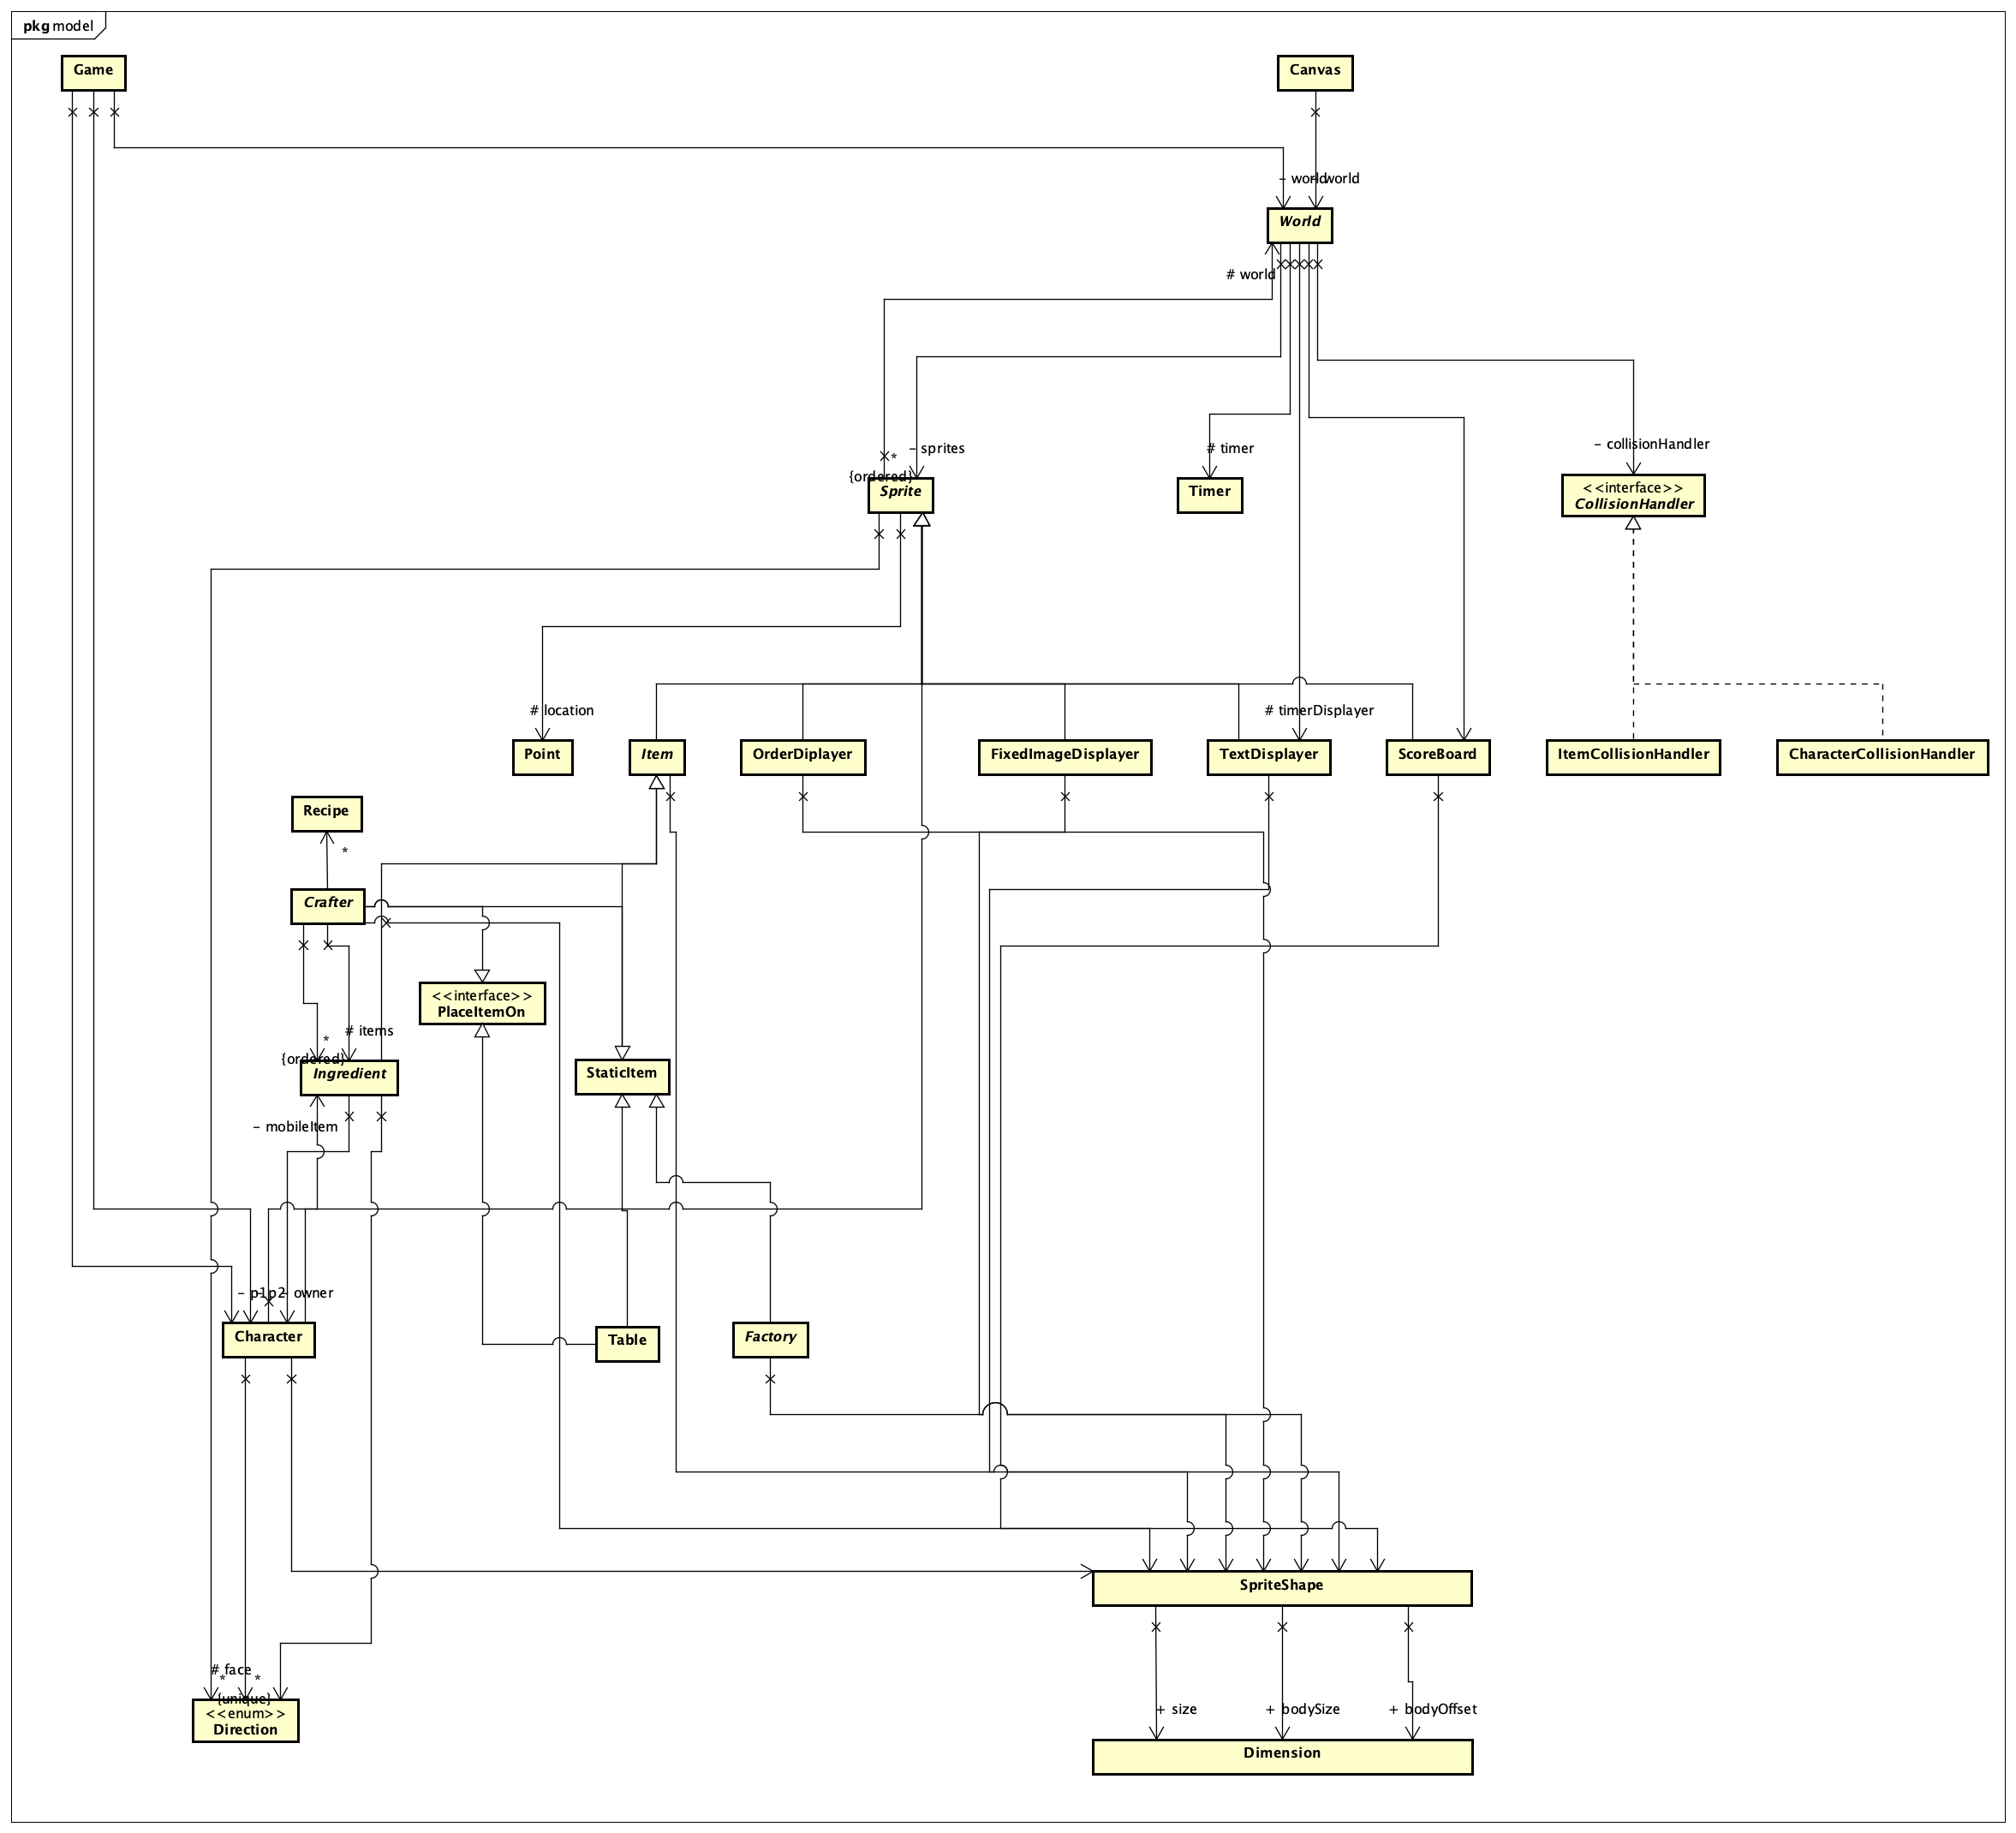
\includegraphics[width=0.8\textwidth]{Model_Class_Diagram}
\caption{Data path of the CPU in this homework.}
\end{figure}


\definecolor{dkgreen}{rgb}{0,0.6,0}
\definecolor{gray}{rgb}{0.5,0.5,0.5}
\definecolor{mauve}{rgb}{0.58,0,0.82}

\lstset{frame=tb,
  language=Java,
  aboveskip=3mm,
  belowskip=3mm,
  showstringspaces=false,
  columns=flexible,
  basicstyle={\small\ttfamily},
  numbers=none,
  numberstyle=\tiny\color{gray},
  keywordstyle=\color{blue},
  commentstyle=\color{dkgreen},
  stringstyle=\color{mauve},
  breaklines=true,
  breakatwhitespace=true,
  tabsize=3
}

\newpage
\section{Advantage of Design}
\begin{enumerate}
\item Open-Closed Principle (OCP) \\
We achieve OCP in \textbf{Ingredient}, \textbf{Recipe}, \textbf{Factory}, \textbf{StaticItem}, \textbf{World}.
    One can add any ingredients by extending the \textbf{Ingredient} class as
\lstinputlisting[language=Java]{1.java}

One can creates any recipe by extending the abstract \textbf{ConcreteRecipe} class
\lstinputlisting[language=Java]{2.java}

One can creates any ingredient factory by extending the abstract \textbf{Factory} class
\lstinputlisting[language=Java]{3.java}

One can creates any static item by extending the abstract \textbf{StaticItem} class public class
\lstinputlisting[language=Java]{4.java}

Finally, one can also creates a customized map and world by extending the abstract \textbf{World} class.
\item Not many outer source code and packages are utilized, make our codes rather "lightweight".
\end{enumerate}

\section{Disadvantage of Design}
\subsection{File IO}
Beacuse we use java.IO.File to access our assets, it is nearly impoosible to package the whole game as a file.
A proper way to load image from .jar file is to use getClassLoader().getResourceAsStream(). However, since the utility is design to load state by
all file name, it is not likely possible to do so.
\subsection{Design limit}
We us java AWT as our GUI engine, and because it is quite old package, some of our design is limited by its ability.

\section{Packages Utilization}
No outer source package other than java AWT is imported in this project. But we can have to attribute and thank TA Waterball for providing the template code for 2D game design in package \textbf{Java-Game-Programming-with-FSM-and-MVC}, especially for the design of \textbf{FiniteStateMachine} packge \textbf{fsm}, and all parts related to image rendering.\\
All picture and icons designs are download from free database \textbf{flaticon}, with attribution to creator \textbf{Freepik}.

\section{How to Play}
After entering the game menu, the player can determine the number of players (1-2) and which game world to play (No.1 – No.5). Then, the player can click the start button to start the game.\\
During the game, one can see that the character(s) and the game map are in the middle of the window. On the right side of the window, there are a timer, a scoreboard, and recipes. The food orders are shown at the bottom of the window, the player can finish the order and get a score by following the recipe to cook the food and deliver it to the pickup window. If the player delivers one food that is not in the orders, he/she would get score punishment by deducting score by 10. The orders would increase during the time and the maximum number of orders is 5.\\
Both players are controlled by the keyboard.
\begin{itemize}
    \item Player1: Move \textbf{W}/\textbf{A}/\textbf{S}/\textbf{D}. Pickup food: \textbf{Q}. Place food: \textbf{E}
    \item Player2: Move \textbf{I}/\textbf{J}/\textbf{K}/\textbf{L}. Pickup food: \textbf{U}. Place food: \textbf{O}
\end{itemize}


In the game, the player(s) can get food ingredients from 7 items. There are \textbf{EggBasket}, \textbf{BreadBasket}, \textbf{CheeseBlock}, \textbf{SpinachGarden}, \textbf{PieBox}, \textbf{FruitBasket} and \textbf{TomatoBasket}.\\
Despite the fact that the \textbf{FruitBasket} can provide random fruit (apple, banana, and orange), others can only provide one kind of food which is simply shown by their names.\\
There are 4 kinds of items where food can be placed.
\begin{enumerate}
	\item \textbf{WoodPlatform} for placing at most one food.
    \item \textbf{TrashCan} for abandoning food.
    \item \textbf{ApplePieStove}, \textbf{SaladBowl}, \textbf{SandwichMaker}, and \textbf{FriedEggStove} for cooking food.
    \item \textbf{PickupWindow} for delivering food.
\end{enumerate}
When time is up, the game would enter the end page and the player could click play again to enter the menu to start a new game.\\
\quad \\




%%%%%%%%%%%%%%%%%%%%%%%%%%%%%%%%%%%%%%%%%%%%%%%%%%%%%%%%%%%%%

\end{document}
